% !TeX program = xelatex
% 编译：xelatex final_slides.tex（两遍）
\documentclass[aspectratio=169,10pt]{ctexbeamer}

\usetheme[progressbar=frametitle]{metropolis}
\metroset{block=fill}
\usepackage{booktabs}
\usepackage{amssymb}
\usepackage{tikz}
\usetikzlibrary{arrows.meta, positioning}

\setsansfont{FiraSans-Light.otf}[BoldFont=FiraSans-SemiBold.otf]
\setmonofont{FiraMono-Regular.otf}[Scale=0.85]
\setCJKsansfont{Microsoft YaHei}[BoldFont={Microsoft YaHei Bold}]
\setCJKmainfont{Microsoft YaHei}[BoldFont={Microsoft YaHei Bold}]

\setbeamertemplate{frame numbering}[fraction]
\setbeamercolor{takeaway}{bg=mLightBrown!12, fg=black!75}

% 底部要点条（仅用于关键结论页）
\newcommand{\takeaway}[1]{%
  \vfill
  \begin{beamercolorbox}[rounded=true, center, sep=6pt]{takeaway}
    \small #1
  \end{beamercolorbox}}

% 大数字
\newcommand{\bignum}[2]{%
  \begin{center}
    {\fontsize{26}{30}\selectfont\textbf{\textcolor{mLightBrown}{#1}}}\\[4pt]
    {\small #2}
  \end{center}}

% 居中大图 + 一句加粗图注（图表主导版式）
\newcommand{\chartcap}[2]{%
  \begin{center}
    \includegraphics[width=0.9\textwidth, height=0.64\textheight, keepaspectratio]{#1}\\[4pt]
    {\small\textbf{\color{black!75} #2}}
  \end{center}}

% 顶部数据条
\newcommand{\statline}[1]{\begin{center}{\large\textbf{\textcolor{mLightBrown}{#1}}}\end{center}}

% 截图：存在则插图，否则虚线占位框
\newcommand{\screenshotbox}[3]{%
  \IfFileExists{#1}{%
    {\setlength{\fboxsep}{0pt}\setlength{\fboxrule}{0.4pt}%
     \fcolorbox{black!30}{white}{\includegraphics[width=\dimexpr\linewidth-0.8pt\relax]{#1}}}%
  }{%
    \begin{tikzpicture}
      \draw[dashed, semithick, black!30] (0,0) rectangle (#2,#3);
      \node[black!40] at (0.5*#2,0.5*#3) {\scriptsize 截图待补充};
    \end{tikzpicture}%
  }%
}

\title{基于 MQTT 的多节点环境监测系统设计}
\subtitle{题目 12 · 面向校园场景的最低成本网络层方案}
\author{胡艺瀚 \quad 孙博宇 \quad 韦煜城 \quad 曾家豪\\[4pt]
  {\small 指导老师：和洁 \quad 傅攀峰 \quad 刘若辰}}
\date{2026 年 6 月 18 日}

\begin{document}

\maketitle

% ============================================================
\begin{frame}[standout]
  一、需求分析
\end{frame}

\begin{frame}{应用场景：智慧校园全域环境监测}
  \vspace{2pt}
  {\footnotesize\color{black!70} 校园绿化带与户外公共区域广，温湿度、光照、土壤墒情、空气质量等参数现靠\textbf{人工抽检}——不实时、覆盖不全。需要一套\textbf{覆盖全校、实时、可扩展}的多节点环境监测。}
  \vspace{12pt}
  \begin{center}
    \begin{tikzpicture}[
        card/.style={draw=mLightBrown!50, rounded corners=4pt, fill=mLightBrown!8, align=center,
                     text width=2.55cm, minimum height=1.95cm, inner sep=5pt, font=\scriptsize}]
      \node[card] (a) {\textbf{温度 · 湿度}\\[5pt]微气候\\环境舒适度};
      \node[card, right=0.35cm of a] (b) {\textbf{光照}\\[5pt]植物生长\\景观照明};
      \node[card, right=0.35cm of b] (c) {\textbf{土壤湿度}\\[5pt]绿化\\按需灌溉};
      \node[card, right=0.35cm of c] (d) {\textbf{可燃气体}\\[5pt]空气质量\\燃气安全};
    \end{tikzpicture}
  \end{center}
  \takeaway{多类环境数据 → 智能灌溉 · 环境分析 · 异常告警，这就是我们要服务的真实需求}
\end{frame}

\begin{frame}{功能需求与系统规模}
  \vspace{8pt}
  \begin{columns}[T]
    \begin{column}{0.52\textwidth}
      \textbf{功能需求}
      {\footnotesize
      \begin{itemize}\itemsep=4pt
        \item 多节点采集/模拟，周期可配置
        \item 统一主题与消息格式，经 Broker 转发
        \item Web 监控端订阅并实时显示
        \item 断线重连与异常分析
      \end{itemize}}
    \end{column}
    \begin{column}{0.44\textwidth}
      \textbf{规模跨度}
      {\footnotesize
      \begin{itemize}\itemsep=4pt
        \item 单实验室 / 楼层：十几～几十节点
        \item 单栋楼 / 院系：上百节点
        \item 校园全域：\textbf{万级节点}
      \end{itemize}}
    \end{column}
  \end{columns}
  \vfill
  \begin{center}\small\color{black!55}
    规模跨度极大——同一套方案要从几十节点平滑覆盖到万级。
  \end{center}
\end{frame}

\begin{frame}{性能与服务质量指标}
  \vspace{2pt}
  \begin{center}{\small\color{black!60} 下列服务质量指标为系统的\textbf{硬性约束}，不随规模扩展或成本优化而放宽。}\end{center}
  \vspace{14pt}
  \begin{center}
    \begin{tikzpicture}[
        kpi/.style={draw=black!22, rounded corners=4pt, fill=black!3, align=center,
                    text width=4.7cm, minimum height=1.85cm, inner sep=5pt}]
      \node[kpi] (a) {{\footnotesize\color{black!60} 消息到达率}\\[6pt]
        {\fontsize{21}{25}\selectfont\textbf{\textcolor{mLightBrown}{$\geq$ 95\%}}}};
      \node[kpi, right=0.7cm of a] (b) {{\footnotesize\color{black!60} 平均传输延迟}\\[6pt]
        {\fontsize{21}{25}\selectfont\textbf{\textcolor{mLightBrown}{$\leq$ 1 s}}}};
      \node[kpi, below=0.6cm of a] (c) {{\footnotesize\color{black!60} 断线重连恢复}\\[6pt]
        {\fontsize{21}{25}\selectfont\textbf{\textcolor{mLightBrown}{$\leq$ 10 s}}}};
      \node[kpi, right=0.7cm of c] (d) {{\footnotesize\color{black!60} 连续运行稳定性}\\[6pt]
        {\fontsize{17}{21}\selectfont\textbf{\textcolor{mLightBrown}{长期无异常}}}};
    \end{tikzpicture}
  \end{center}
\end{frame}

\begin{frame}{纳入成本：从“做最强”到“做最省”}
  \vspace{2pt}
  {\small\color{black!60} 中期检查时老师指出：不要只追求“最强”，方案必须考虑\textbf{成本}。}
  \vspace{8pt}
  \begin{columns}[c, onlytextwidth]
    \begin{column}{0.44\textwidth}
      \centering
      \begin{tikzpicture}
        \node[draw=red!45, line width=0.7pt, rounded corners=5pt, fill=red!4,
              text width=0.84\linewidth, align=center, inner sep=10pt, minimum height=2.5cm]
          {{\large\color{red!60!black}\textbf{$\times$\;不追求}}\\[8pt]
           {\footnotesize 最大并发 · 最强性能\\[2pt]“最好的东西”}};
      \end{tikzpicture}
    \end{column}
    \begin{column}{0.10\textwidth}
      \centering {\huge\color{mLightBrown!80}$\Rightarrow$}
    \end{column}
    \begin{column}{0.44\textwidth}
      \centering
      \begin{tikzpicture}
        \node[draw=mLightBrown, line width=0.8pt, rounded corners=5pt, fill=mLightBrown!12,
              text width=0.84\linewidth, align=center, inner sep=10pt, minimum height=2.5cm]
          {{\large\color{mLightBrown}\textbf{\checkmark\;我们追求}}\\[8pt]
           {\footnotesize 覆盖需求 + QoS 达标的\\[2pt]\textbf{最低成本}}};
      \end{tikzpicture}
    \end{column}
  \end{columns}
  \vspace{12pt}
  \begin{alertblock}{我们对成本的核心思考}
    把“做系统”重定义成\,\textbf{“求一个有约束的最小值”}。\\[5pt]
    {\footnotesize\color{black!55} 成本边界：只研究网络层服务器（带宽 / CPU / 内存 / 存储），传感器硬件与供电不纳入本阶段。}
  \end{alertblock}
\end{frame}

% ============================================================
\begin{frame}[standout]
  二、方案设计与实测验证
\end{frame}

\begin{frame}{为什么选 MQTT：与 HTTP 的对比}
  \vspace{8pt}
  {\footnotesize
  \begin{itemize}\itemsep=8pt
    \item \textbf{发布 / 订阅}：Broker 主动推送，实时、天然多对多（HTTP 靠客户端轮询）
    \item \textbf{报文头极小 + 长连接复用}：每条只带极小协议头（HTTP 每条都重发整套头，还可能重建连接）
    \item \textbf{持久会话 + QoS + 重连}：断线可补发、可感知离线（HTTP 无状态，需自行实现）
  \end{itemize}}
  \vspace{2pt}
  \begin{beamercolorbox}[rounded=true, sep=7pt]{takeaway}
    \begin{center}
      {\footnotesize\textbf{实测 · 上传同一条数据的应用层字节（N = 200）}}\\[5pt]
      {\scriptsize
      \setlength{\tabcolsep}{9pt}\renewcommand{\arraystretch}{1.2}
      \begin{tabular}{@{}l r r r@{}}
        \textbf{payload 格式} & \textcolor{mLightBrown}{\textbf{MQTT}} & \textbf{HTTP} & \textbf{MQTT 省} \\
        json（122 B）    & 163 B & 463 B & 65\,\% \\
        json-min（65 B） & 105 B & 405 B & 74\,\% \\
        msgpack（49 B）  & 89 B  & 392 B & 77\,\% \\
      \end{tabular}}\\[5pt]
      {\footnotesize 协议头开销恒定：MQTT 约 \textbf{40 B} vs HTTP 约 \textbf{340 B}（约 1/8）；数据越小，MQTT 越省。}
    \end{center}
  \end{beamercolorbox}
\end{frame}

\begin{frame}{系统总体架构}
  \vspace{10pt}
  \begin{center}
    \begin{tikzpicture}[
        box/.style={draw=black!50, line width=0.5pt, rounded corners=2pt, fill=black!4,
                    align=center, minimum height=0.9cm, inner sep=6pt, font=\small},
        hub/.style={box, fill=mLightBrown!12, draw=mLightBrown},
        arr/.style={-{Stealth[length=2.2mm]}, black!55, semithick}
      ]
      \node[box] (n1) {ESP32 硬件节点};
      \node[box, below=0.3cm of n1] (n2) {PC 模拟节点 $\times N$};
      \node[hub, right=2.0cm of n1.east, yshift=-0.55cm, minimum height=1.1cm] (broker) {EMQX Broker\\\scriptsize 网络层};
      \node[box, right=2.0cm of broker, minimum height=1.1cm] (web) {Web 监控端\\需求计算器};
      \draw[arr] (n1.east) -- (broker);
      \draw[arr, dashed] (n2.east) -- (broker);
      \draw[arr] (broker) -- node[above, font=\tiny\ttfamily, black!50] {subscribe} (web);
      \node[font=\scriptsize, black!55, below=0.05cm of n2] {感知层 N 节点};
    \end{tikzpicture}
  \end{center}
  \vfill
  \begin{center}\small\color{black!55}
    节点接口统一 —— ESP32 与模拟节点同构接入，监控端不区分数据来源。
  \end{center}
\end{frame}

\begin{frame}{协议设计：为降负载而生}
  \vspace{2pt}
  \begin{center}
    \begin{tikzpicture}
      \node[fill=mLightBrown!10, draw=mLightBrown!60, rounded corners=3pt,
            inner xsep=12pt, inner ysep=6pt]
        {\small\texttt{env\_monitor/\{node\_id\}/\{data\_type\}}};
    \end{tikzpicture}
  \end{center}
  \vspace{10pt}
  {\footnotesize
  \begin{itemize}\itemsep=6pt
    \item \textbf{压 payload}：json $\to$ json-min $\to$ msgpack，单条 261.9 $\to$ 203.0 $\to$ 185.9 B
    \item \textbf{省主题}：MQTT 5.0 Topic Alias，每条再省 21.3 B
    \item \textbf{QoS 够用即可}：上报选 QoS 1，不盲目上 QoS 2
  \end{itemize}}
  \vspace{6pt}
  \hfill{\footnotesize\color{mLightBrown}\textbf{→ 每个选择都指向更少字节、更低配置}}
\end{frame}

\begin{frame}{实测佐证 · 协议开销}
  \chartcap{images/exp_overhead.png}{json / json-min / msgpack = 261.9 / 203.0 / 185.9 B · Topic Alias 每条省 21.3 B}
\end{frame}

\begin{frame}{Broker 选型：EMQX 单机扛万级（实测）}
  \vspace{4pt}
  \begin{columns}[c]
    \begin{column}{0.38\textwidth}
      {\footnotesize
      \begin{itemize}\itemsep=10pt
        \item \textbf{内存}：amqtt 仅在约 1 万连接（~500 MB）以下略省，而内存普遍 \textbf{2 GB 起步}，这点差距可忽略
        \item \textbf{CPU}：EMQX \textbf{全段占优}，amqtt 5 万连接时单核打满
        \item \textbf{扩容}：EMQX 支持集群横向扩展，amqtt 单机单核难扩
      \end{itemize}}
    \end{column}
    \begin{column}{0.60\textwidth}
      \centering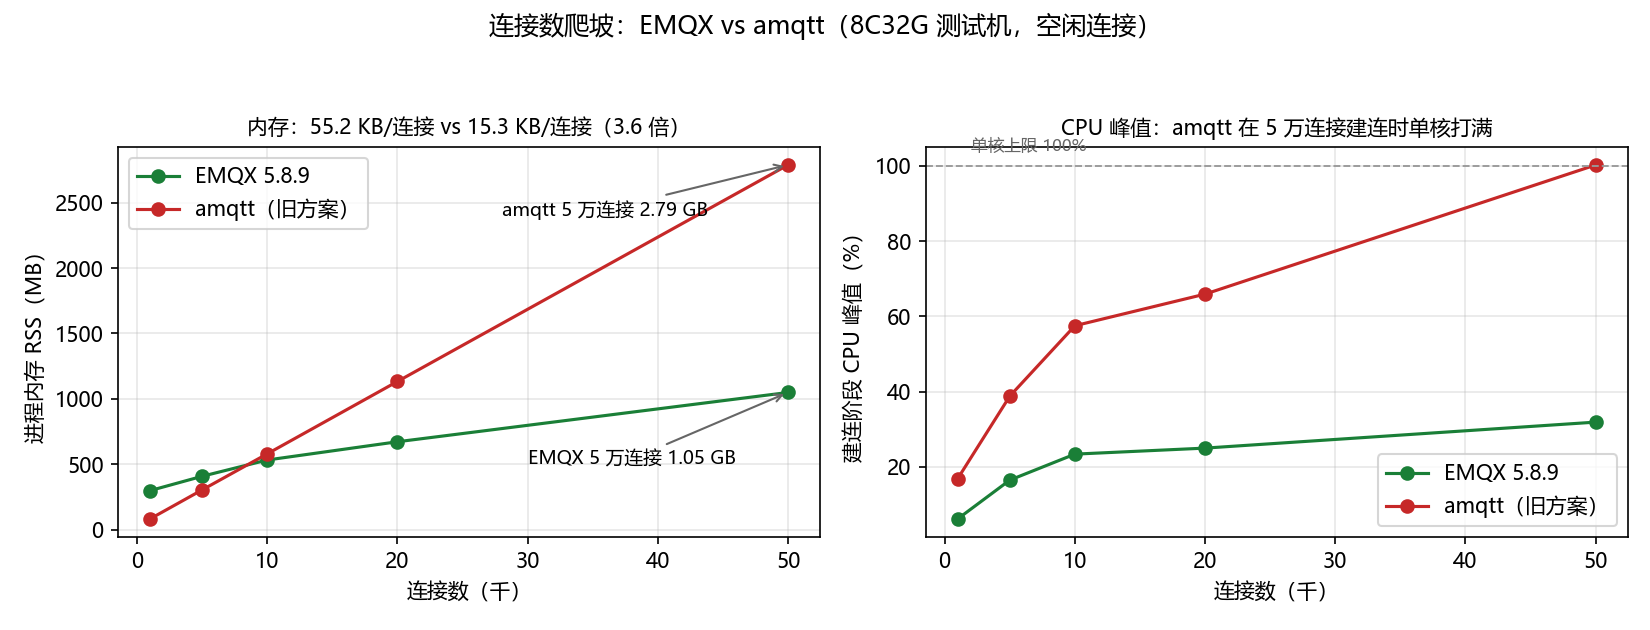
\includegraphics[width=\linewidth, height=0.66\textheight, keepaspectratio]{images/exp_capacity.png}
    \end{column}
  \end{columns}
  \takeaway{内存的微弱差距可忽略，CPU 与扩容 EMQX 全面占优 —— 面向万级，选 EMQX}
\end{frame}

\begin{frame}{实测佐证 · 吞吐}
  \vspace{2pt}
  \begin{columns}[c]
    \begin{column}{0.64\textwidth}
      \centering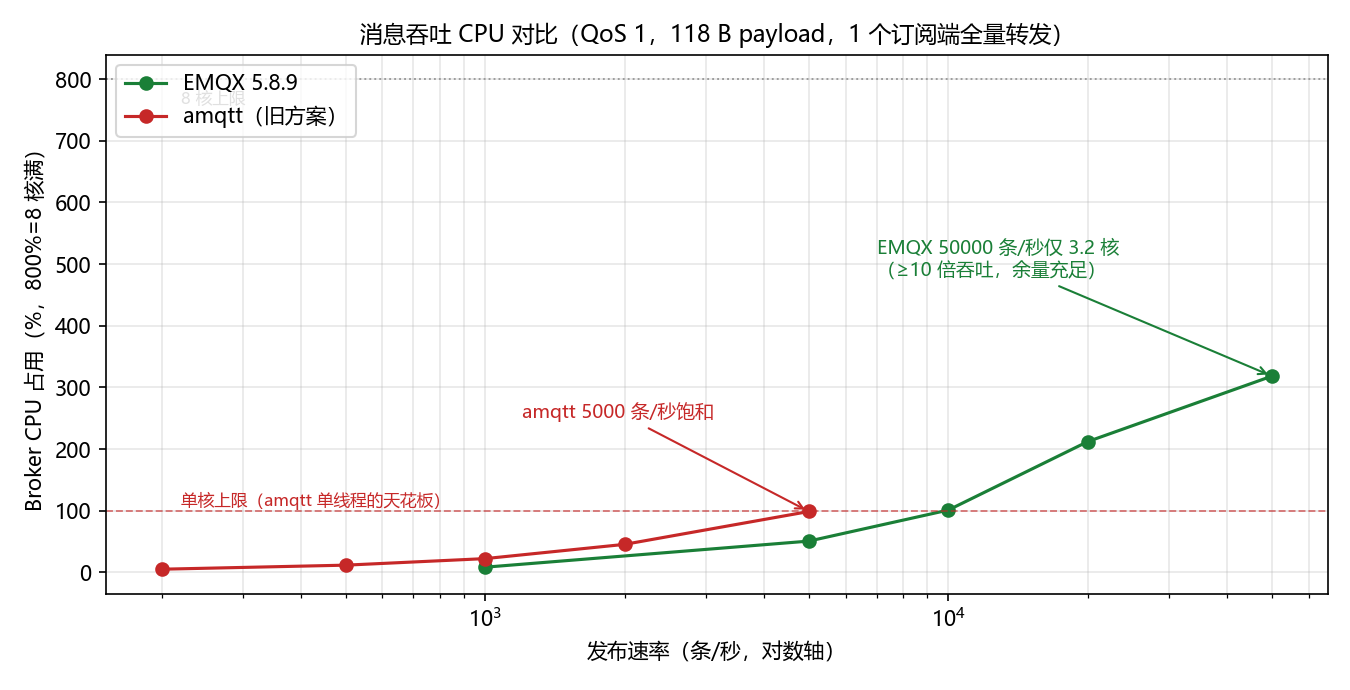
\includegraphics[width=\linewidth, height=0.66\textheight, keepaspectratio]{images/exp_throughput.png}
    \end{column}
    \begin{column}{0.34\textwidth}
      \bignum{5 万条/秒}{EMQX 仅用 3.2 核\\ 19000 条/核·s}
    \end{column}
  \end{columns}
\end{frame}

\begin{frame}{服务质量保障：QoS 1 + 持久会话 + 重连}
  \vspace{4pt}
  {\footnotesize\color{black!60} TCP 已保证\textbf{连接内}不丢包；QoS 要解决的是\textbf{连接断开}（broker 重启 / 节点掉线重连）时消息不丢。}
  \vspace{10pt}
  \begin{center}
    \begin{tikzpicture}[
        card/.style={draw=mLightBrown!55, rounded corners=4pt, fill=mLightBrown!8, align=center,
                     text width=3.3cm, minimum height=2.5cm, inner sep=8pt}]
      \node[card] (a) {{\large\textbf{QoS 1}}\\[8pt]{\footnotesize\color{black!70} 至少一次送达\\离线消息排队补发}};
      \node[card, right=0.6cm of a] (b) {{\large\textbf{持久会话}}\\[8pt]{\footnotesize\color{black!70} 固定 client\_id\\断线期间消息不丢}};
      \node[card, right=0.6cm of b] (c) {{\large\textbf{自动重连}}\\[8pt]{\footnotesize\color{black!70} 断网恢复后续传\\无需人工干预}};
    \end{tikzpicture}
  \end{center}
  \takeaway{QoS 1（至少一次）+ 持久会话扛掉线重连；重复由 \texttt{seq} 去重，无需 QoS 2 —— 不丢、不重、还省}
\end{frame}

\begin{frame}{实测佐证 · QoS × 丢包}
  \vspace{2pt}
  \begin{columns}[c]
    \begin{column}{0.34\textwidth}
      \bignum{100\%}{0–15\% 丢包下\\ 三种 QoS 到达率\\ 均 100\%（靠 TCP 重传）}
    \end{column}
    \begin{column}{0.64\textwidth}
      \centering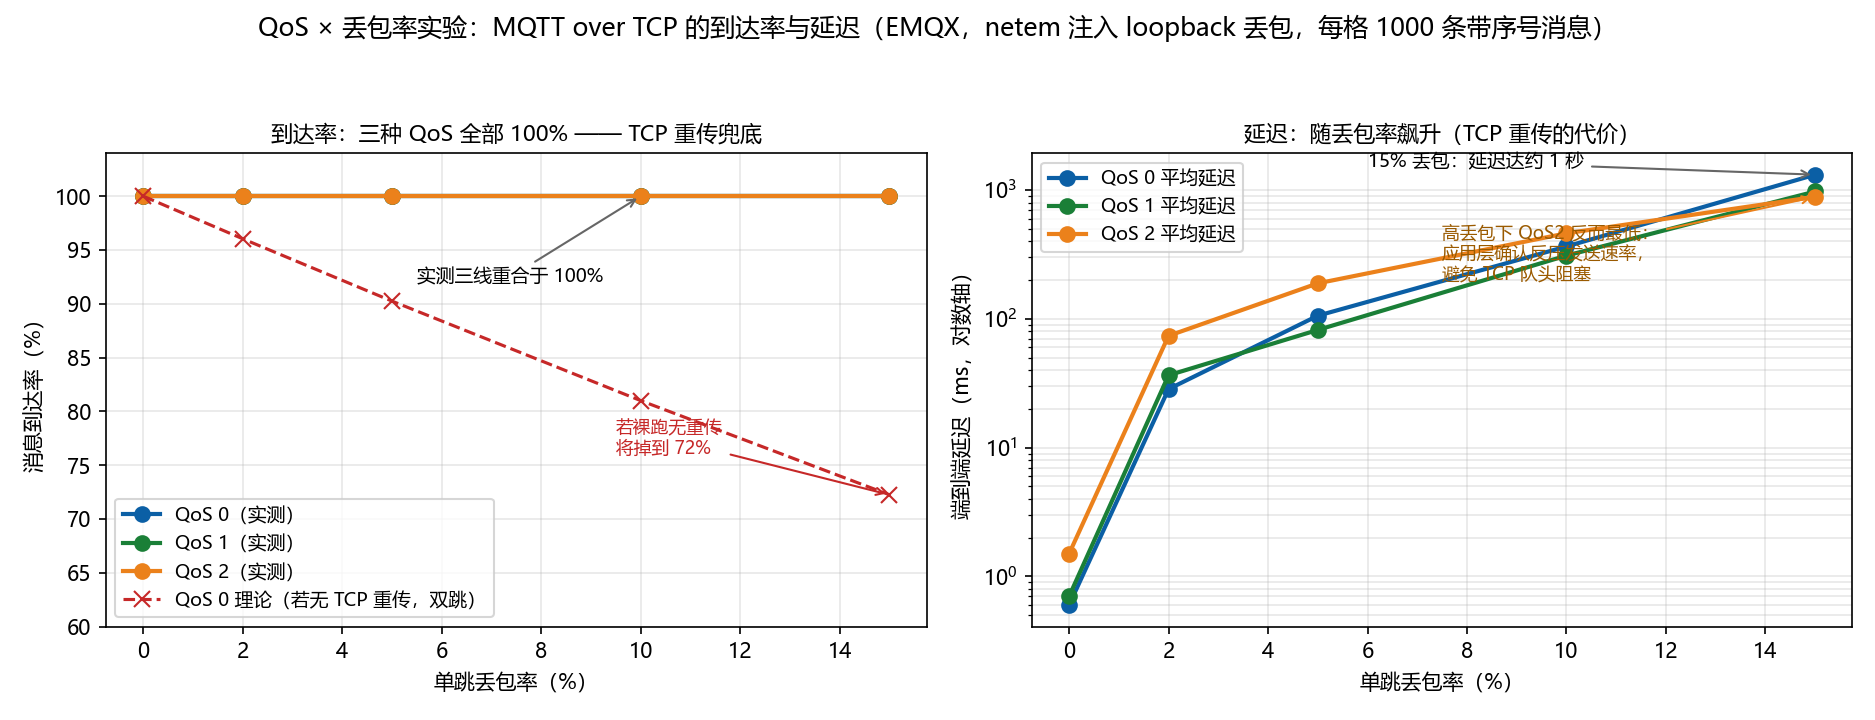
\includegraphics[width=\linewidth, height=0.66\textheight, keepaspectratio]{images/exp_qos_loss.png}
    \end{column}
  \end{columns}
  \takeaway{三种 QoS 都 100\%，恰恰说明\textbf{抗丢包是 TCP 的事、不是 QoS 的事}；QoS 的价值在\textbf{断连}场景 —— 故选 QoS 1 + 持久会话（跨公网重连 5.2 s 仍零丢失）}
\end{frame}

\begin{frame}{实测佐证 · 跨公网延迟}
  \statline{平均 44.7 ms \quad·\quad 到达率 100\% \quad·\quad 断线重连 5.2 s}
  \vspace{2pt}
  \begin{center}
    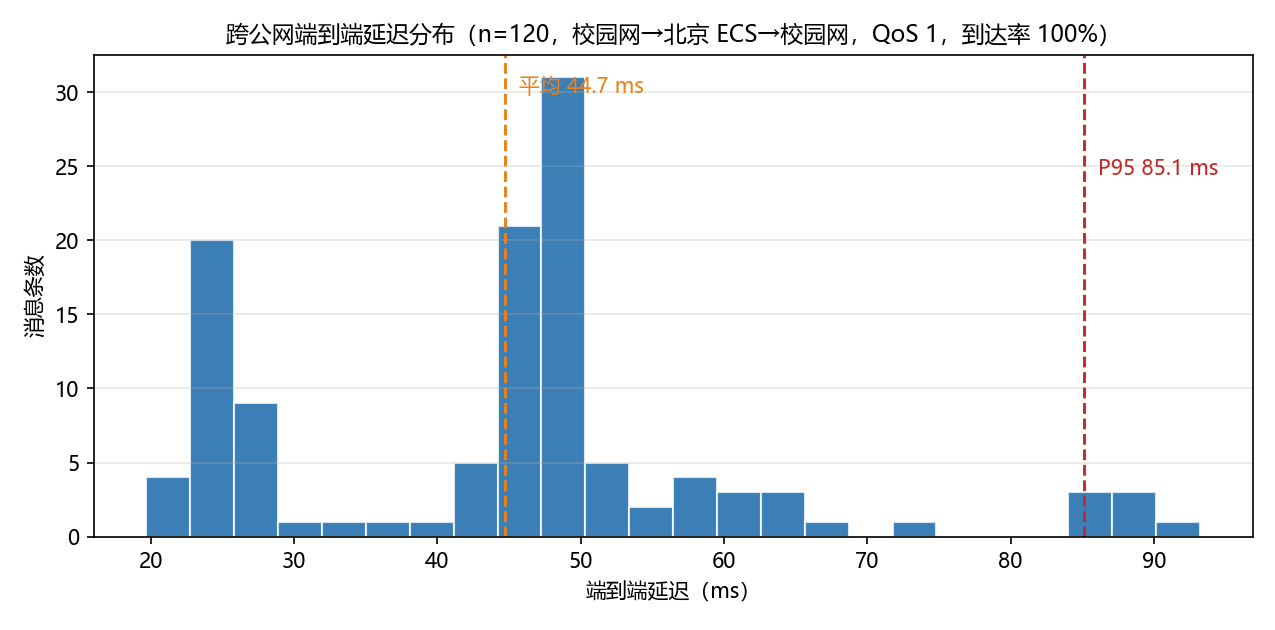
\includegraphics[width=0.82\textwidth, height=0.58\textheight, keepaspectratio]{images/exp_latency.png}
  \end{center}
\end{frame}

\begin{frame}{求“最小资源”的方法}
  \vspace{16pt}
  \begin{center}
    \begin{tikzpicture}[
        b/.style={draw=black!45, rounded corners=2pt, fill=black!4, align=center,
                  minimum height=1.0cm, inner sep=5pt, font=\scriptsize},
        a/.style={-{Stealth[length=2mm]}, black!55, semithick}]
      \node[b] (p1) {需求参数\\$N,M,T,$QoS};
      \node[b, right=0.7cm of p1] (p2) {网络负载\\带宽·流量};
      \node[b, right=0.7cm of p2] (p3) {满足 QoS 的\\最小配置};
      \node[b, right=0.7cm of p3] (p4) {成本};
      \draw[a] (p1) -- (p2); \draw[a] (p2) -- (p3); \draw[a] (p3) -- (p4);
      \node[font=\tiny, mLightBrown, below=0.12cm of p2] {抓包标定};
      \node[font=\tiny, mLightBrown, below=0.12cm of p3] {压测标定};
    \end{tikzpicture}
  \end{center}
  \vfill
  \begin{center}\small\color{black!55}
    关键：用实验把“每连接/每消息”的系数测准，才能算出不多不少的最小配置。
  \end{center}
\end{frame}

\begin{frame}{实测佐证 · 内存双模型}
  \chartcap{images/exp_memory.png}{满负载每连接内存 38.76 KB，是空闲的 2.46 倍 —— 选型必须按满负载上界}
\end{frame}

\begin{frame}{资源计算器：把方法固化成工具}
  \vspace{6pt}
  \begin{center}
    \begin{tikzpicture}[
        io/.style={draw=black!40, rounded corners=3pt, fill=black!4, align=center,
                   font=\scriptsize, inner sep=6pt, minimum height=1.15cm, text width=3.0cm},
        tool/.style={draw=mLightBrown, line width=0.6pt, fill=mLightBrown!15, rounded corners=3pt,
                     align=center, font=\small, inner sep=6pt, minimum height=1.15cm, text width=2.1cm},
        a/.style={-{Stealth[length=2.6mm]}, black!55, semithick}]
      \node[io] (in) {\textbf{输入需求}\\[2pt] 节点数 · 类型 · 周期\\ QoS · 格式 · 订阅端};
      \node[tool, right=0.8cm of in] (t) {\textbf{资源计算器}};
      \node[io, right=0.8cm of t] (out) {\textbf{输出方案}\\[2pt] 带宽 · 月流量 · 磁盘\\ \textbf{服务器最小配置} · 成本};
      \draw[a] (in) -- (t);
      \draw[a] (t) -- (out);
    \end{tikzpicture}
  \end{center}
  \vspace{10pt}
  \begin{center}
    \begin{minipage}{0.80\textwidth}
      \screenshotbox{images/calculator.png}{11.0cm}{4.0cm}
    \end{minipage}
  \end{center}
\end{frame}

\begin{frame}{ESP32-C3 硬件节点：组成与传感器接入}
  \vspace{2pt}
  \begin{columns}[T]
    \begin{column}{0.40\textwidth}
      \textbf{\footnotesize 传感器接入（模块化、可扩展）}\\[3pt]
      {\scriptsize
      \begin{tabular}{@{}lll@{}}
        \toprule
        传感器 & 接口 & 采集量 \\
        \midrule
        DHT11 & GPIO5 & 温度 · 湿度 \\
        BH1750 & I2C (GPIO1/2) & 光照 \\
        FC-28 & GPIO3 & 土壤湿度 \\
        MQ-2 & GPIO4 & 可燃气体 \\
        \bottomrule
      \end{tabular}}\\[5pt]
      {\scriptsize\color{black!50} 每类传感器独立采集函数、主程序统一调度，新增传感器不动主结构。}
    \end{column}
    \begin{column}{0.58\textwidth}
      \centering
      \textbf{\footnotesize 开发板与传感器整体接线}\\[2pt]
      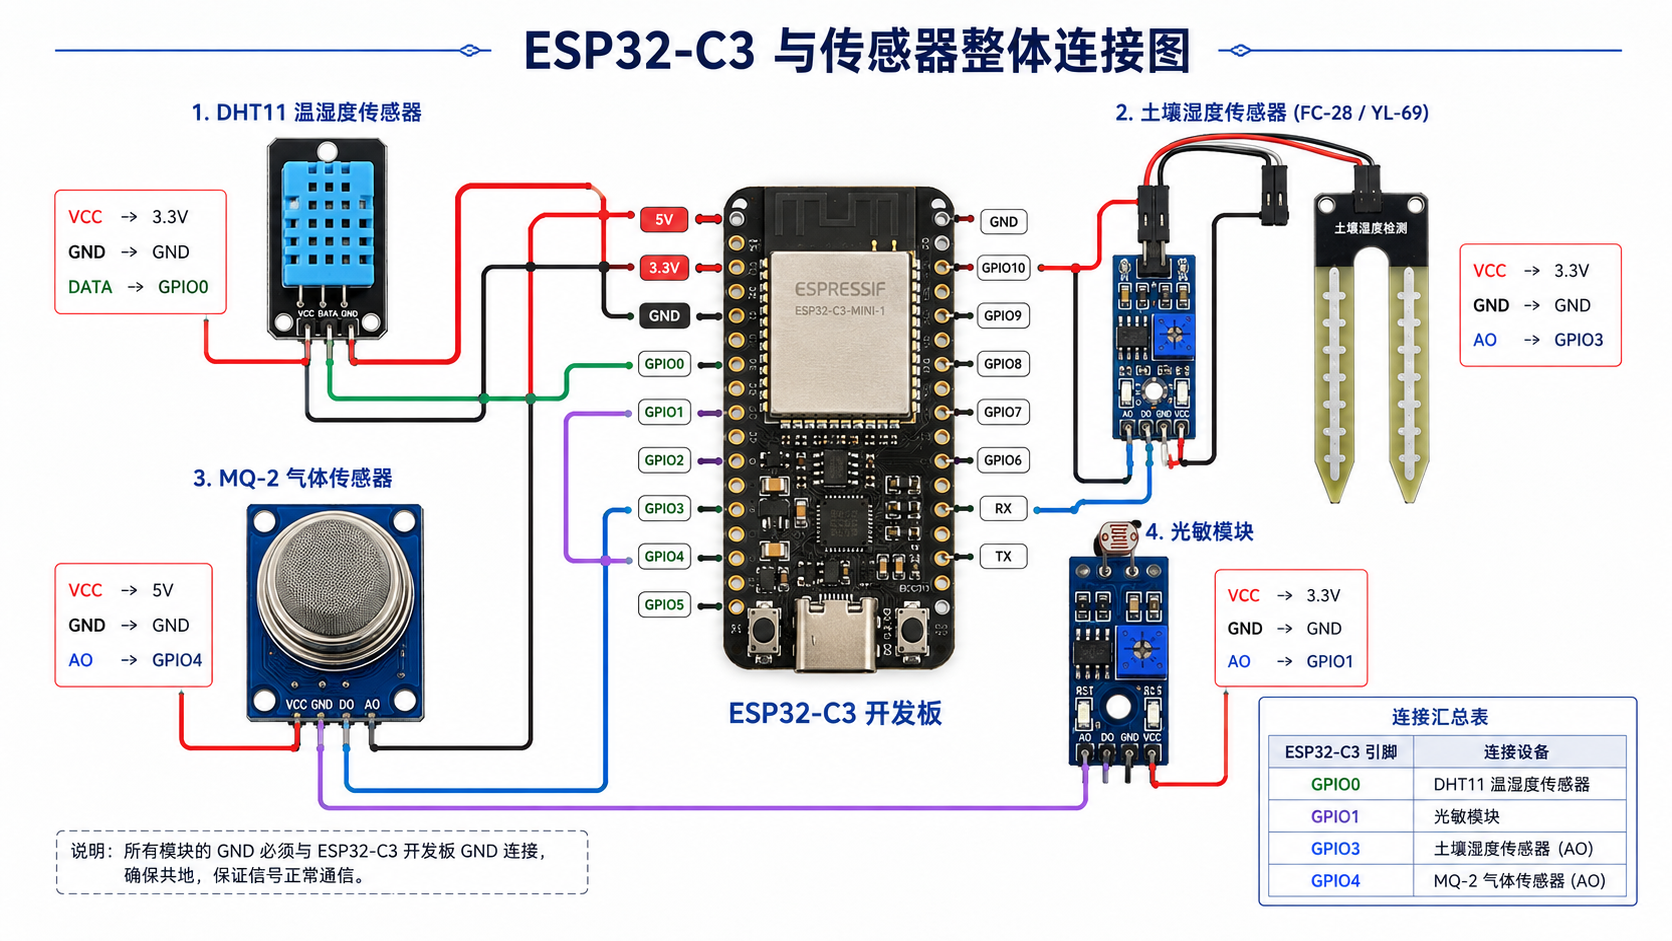
\includegraphics[width=\linewidth, height=0.50\textheight, keepaspectratio]{images/hw_wiring.png}
    \end{column}
  \end{columns}
  \vspace{4pt}
  \begin{center}
    \begin{tikzpicture}[
        b/.style={draw=black!50, rounded corners=2pt, fill=black!4, align=center,
                  font=\scriptsize, minimum height=0.6cm, minimum width=1.32cm, inner sep=1pt},
        hub/.style={b, fill=mLightBrown!12, draw=mLightBrown},
        a/.style={-{Stealth[length=1.6mm]}, black!55, semithick}]
      \node[b] (s1) {启动};
      \node[b, right=0.22cm of s1] (s2) {初始化};
      \node[b, right=0.22cm of s2] (s3) {连 Wi-Fi};
      \node[b, right=0.22cm of s3] (s4) {NTP};
      \node[hub, right=0.22cm of s4] (s5) {连 MQTT};
      \node[b, right=0.22cm of s5] (s6) {周期采集};
      \node[b, right=0.22cm of s6] (s7) {JSON};
      \node[b, right=0.22cm of s7] (s8) {发布};
      \draw[a] (s1)--(s2);\draw[a] (s2)--(s3);\draw[a] (s3)--(s4);\draw[a] (s4)--(s5);
      \draw[a] (s5)--(s6);\draw[a] (s6)--(s7);\draw[a] (s7)--(s8);
    \end{tikzpicture}\\[3pt]
    {\scriptsize\color{black!55} 硬件节点程序流程：Wi-Fi 与 NTP 就绪后才上传带时间戳数据；断网 / MQTT 断开自动重连续传}
  \end{center}
\end{frame}

\begin{frame}{Wi-Fi 配网与网络接入}
  \vspace{2pt}
  \begin{columns}[c]
    \begin{column}{0.54\textwidth}
      \centering\textbf{\footnotesize WiFiManager 配网流程}\\[4pt]
      \begin{tikzpicture}[node distance=3.2mm,
          b/.style={draw=black!50, rounded corners=2pt, fill=black!4, align=center, font=\tiny, text width=3.4cm, inner sep=3pt},
          d/.style={draw=mLightBrown, fill=mLightBrown!14, align=center, font=\tiny, text width=2.0cm, inner sep=3pt},
          ap/.style={draw=black!50, rounded corners=2pt, fill=black!4, align=center, font=\tiny, text width=3.0cm, inner sep=3pt},
          a/.style={-{Stealth[length=1.6mm]}, black!55, semithick}]
        \node[b] (n1) {系统启动 → 初始化 Wi-Fi 配网模块};
        \node[b, below=of n1] (n2) {尝试连接已保存 Wi-Fi};
        \node[d, below=of n2] (n3) {连接成功？};
        \node[b, below=of n3] (n4) {输出 IP / 网关 / RSSI\\ → NTP 同步 → MQTT 连接 → 周期上传};
        \node[ap, right=1.0cm of n3] (m1) {开启 ESP32C3\_Config 热点\\ → 访问 192.168.4.1 选 Wi-Fi\\ → 保存并连接目标网络};
        \draw[a] (n1)--(n2); \draw[a] (n2)--(n3);
        \draw[a] (n3)-- node[left, font=\tiny, black!55] {是} (n4);
        \draw[a] (n3)-- node[above, font=\tiny, black!55] {否} (m1);
        \draw[a] (m1) |- (n2);
      \end{tikzpicture}
    \end{column}
    \begin{column}{0.44\textwidth}
      \centering
      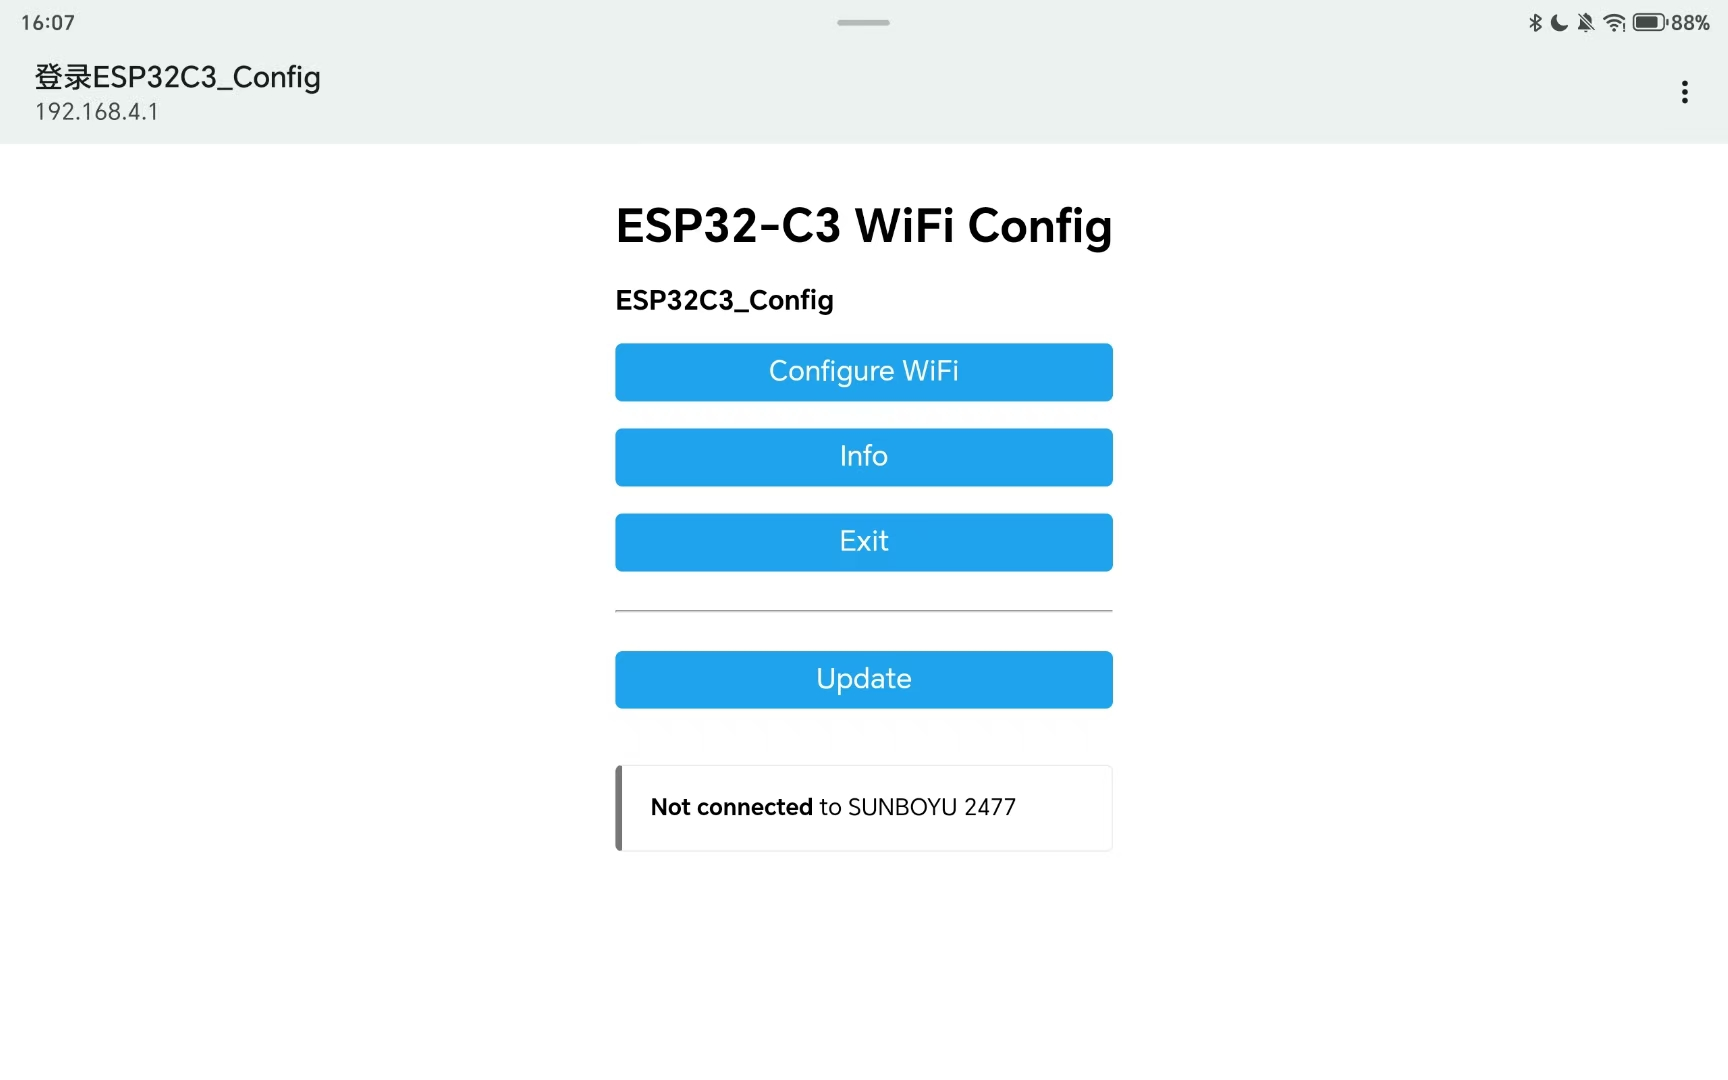
\includegraphics[width=0.72\linewidth, height=0.36\textheight, keepaspectratio]{images/hw_portal1.jpg}\\[2pt]
      {\scriptsize\color{black!55} 配网门户：网页选择 Wi-Fi}\\[6pt]
      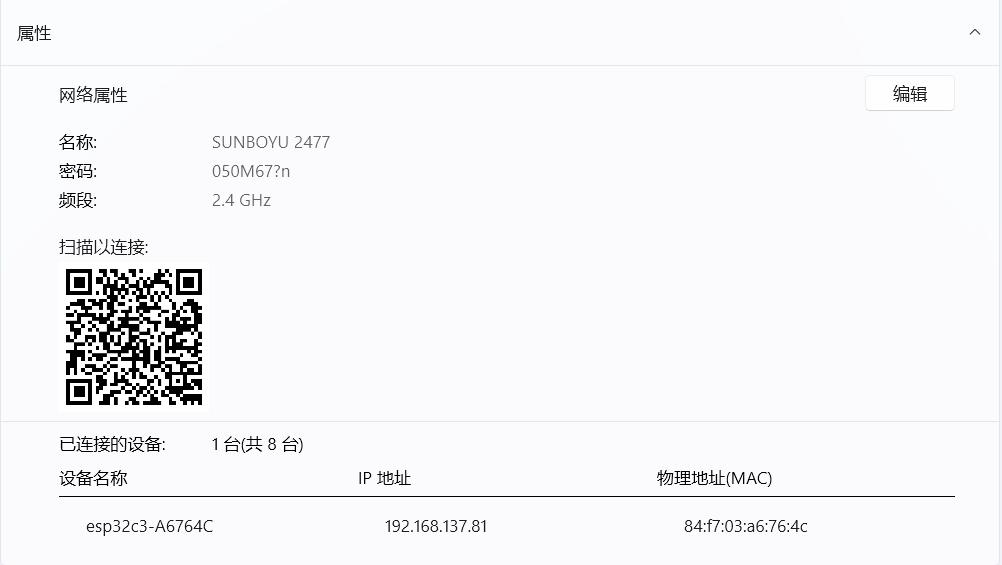
\includegraphics[width=\linewidth, height=0.24\textheight, keepaspectratio]{images/hw_wifi_ok.png}\\[2pt]
      {\scriptsize\color{black!55} 成功接入：ESP32 获 192.168.137.81}
    \end{column}
  \end{columns}
  \takeaway{WiFiManager 配网机制解决了固定 Wi-Fi 不便维护的问题，使 ESP32-C3 节点具备换网配置、自动连接与断线恢复能力}
\end{frame}

\begin{frame}{整链路真机验证 · ESP32 长时测试}
  \vspace{2pt}
  \begin{columns}[T]
    \begin{column}{0.33\textwidth}\bignum{$\sim$15 h}{连续运行零重启}\end{column}
    \begin{column}{0.33\textwidth}\bignum{8547 条}{真机上报}\end{column}
    \begin{column}{0.33\textwidth}\bignum{95\%}{到达率}\end{column}
  \end{columns}
  \begin{center}
    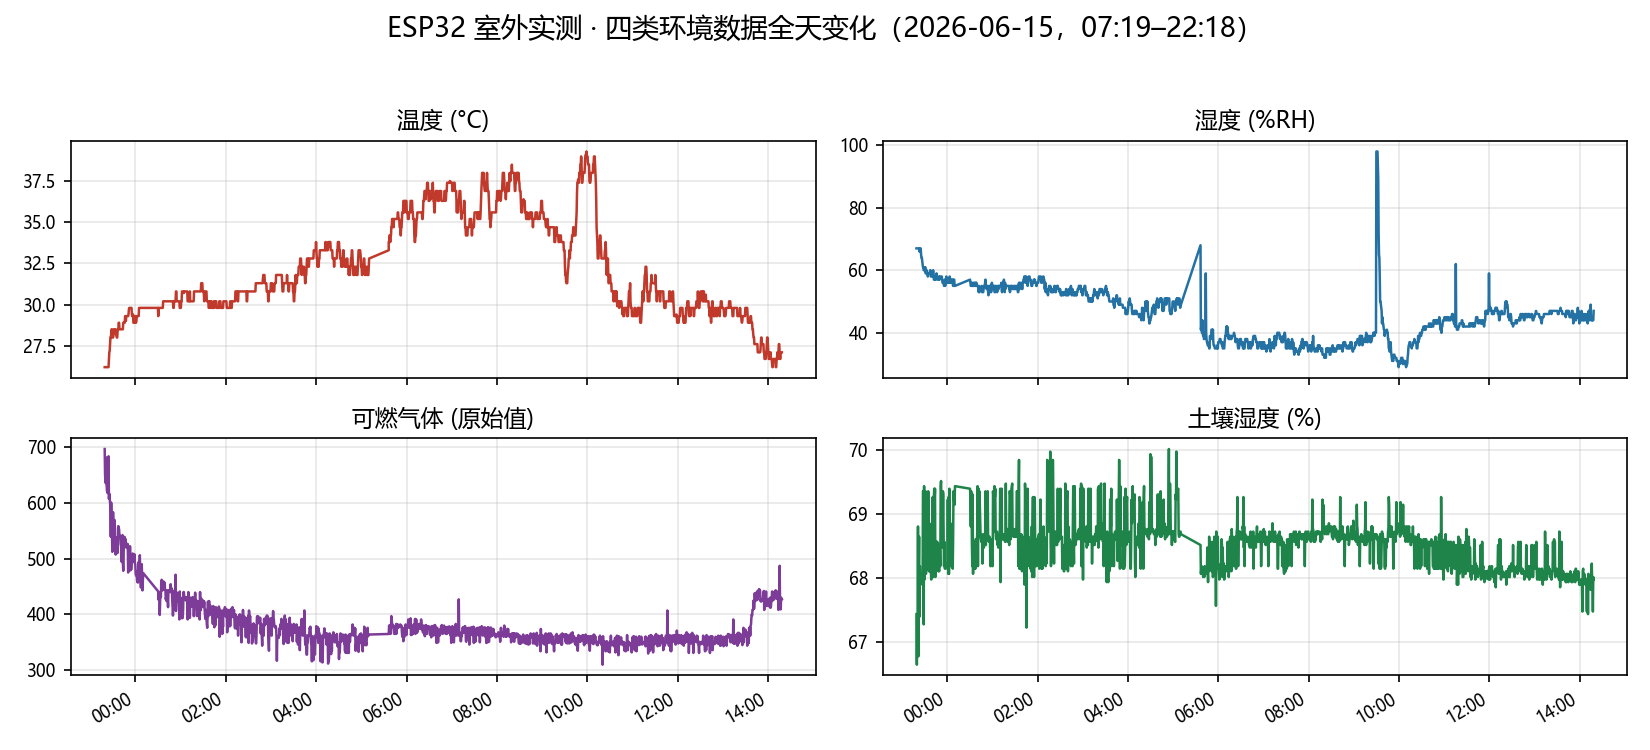
\includegraphics[width=0.78\textwidth, height=0.36\textheight, keepaspectratio]{images/esp32_sensors.png}
  \end{center}
  \takeaway{温度日变化与当天西安天气吻合 · QoS1+持久会话让 2 次网络中断自动续传、零丢失}
\end{frame}

\begin{frame}{光照实测与硬件工程改进}
  \vspace{2pt}
  \begin{columns}[c]
    \begin{column}{0.61\textwidth}
      \centering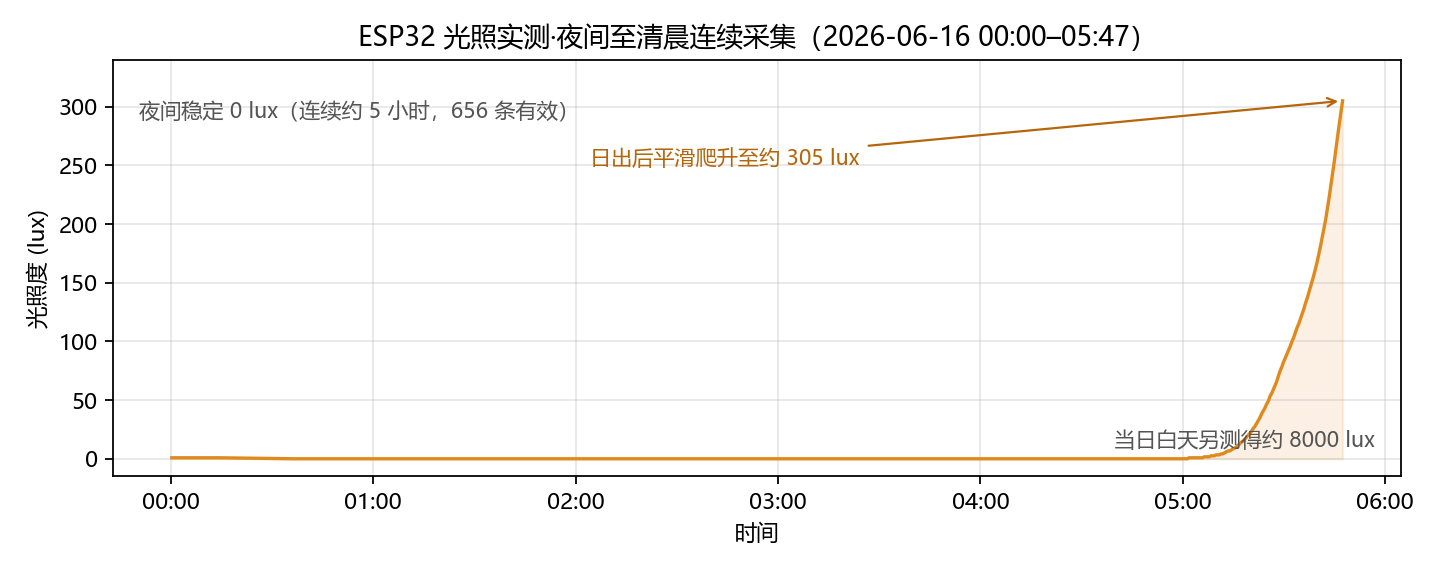
\includegraphics[width=\linewidth, height=0.50\textheight, keepaspectratio]{images/light_dawn.png}
    \end{column}
    \begin{column}{0.37\textwidth}
      \textbf{\footnotesize 工程改进（问题 → 措施）}
      {\scriptsize
      \begin{itemize}\itemsep=5pt
        \item 接线接触不稳 → 重新整理共地、加有效性判断
        \item 写死 Wi-Fi → 引入 AP 配网（WiFiManager）
        \item MQTT 断连 → 连接状态检测 + 自动重连
      \end{itemize}}
    \end{column}
  \end{columns}
  \takeaway{BH1750 经 I2C 采集：夜间至清晨连续 6 小时有效，日出爬升至 305 lux、白天约 8000 lux}
\end{frame}

% ============================================================
\begin{frame}[standout]
  三、具体案例
\end{frame}

\begin{frame}{案例：校园每 100\,m$^2$ 一个节点}
  \vspace{6pt}
  \begin{columns}[c]
    \begin{column}{0.54\textwidth}
      \footnotesize
      \begin{itemize}\itemsep=7pt
        \item 渭水校区约 \textbf{200 万 m$^2$}
        \item 每 100\,m$^2$ 布一个监测节点
        \item $\Rightarrow$ \textbf{约 2 万个节点（万级）}
        \item 参数：4 类 · 60 s · QoS 1 · json-min · 10 监控端
      \end{itemize}
    \end{column}
    \begin{column}{0.42\textwidth}
      \centering
      \begin{tikzpicture}[scale=0.62]
        \draw[black!30, rounded corners=3pt] (0,0) rectangle (6,3.6);
        \foreach \x in {0.6,1.4,...,5.5}
          \foreach \y in {0.5,1.3,...,3.2}
            \fill[mLightBrown] (\x,\y) circle (1.1pt);
        \node[font=\tiny, black!55] at (3,-0.5) {每格 100\,m$^2$ 一节点 · ≈ 2 万};
      \end{tikzpicture}
    \end{column}
  \end{columns}
\end{frame}

\begin{frame}{现场算：这个案例要多大服务器？}
  \vspace{2pt}
  \begin{columns}[c]
    \begin{column}{0.50\textwidth}
      {\small
      \begin{tabular}{ll}
        \toprule
        指标 & 计算器输出 \\
        \midrule
        消息率 R & 1333 条/s \\
        总流量 W & 26.4 Mbps \\
        月流量 & 8.6 TB \\
        磁盘（30 天） & 345 GB \\
        \textbf{服务器} & \textbf{2核4G} \\
        \bottomrule
      \end{tabular}}
    \end{column}
    \begin{column}{0.46\textwidth}
      \bignum{1 台}{2核4G 迷你主机（约 ¥600–1000）\\ 撑起全校 2 万节点}
    \end{column}
  \end{columns}
  \vspace{8pt}
  \begin{block}{可行性校验：瓶颈在带宽与存储，但都够用}
    \footnotesize
    \textcolor{mLightBrown}{\checkmark}~\textbf{带宽}：需求 26.4 Mbps（留余量 ~33）< 校园网 \textbf{100 Mbps}，约 1/3 占用\\[3pt]
    \textcolor{mLightBrown}{\checkmark}~\textbf{存储}：约 11.5 GB/天，30 天 \textbf{345 GB} → 配 ≥400 GB 盘（保留更久则降采样）
  \end{block}
\end{frame}

\begin{frame}{实测佐证 · 实景压测（1/2）：连接零掉线 · 转发满速}
  {\footnotesize\color{black!60} 正是按本案例规模（2 万连接）做的实景压测：}
  \statline{2 万连接 \quad·\quad 30 min 零掉线 \quad·\quad 送达 99.96\%}
  \vspace{2pt}
  \begin{center}
    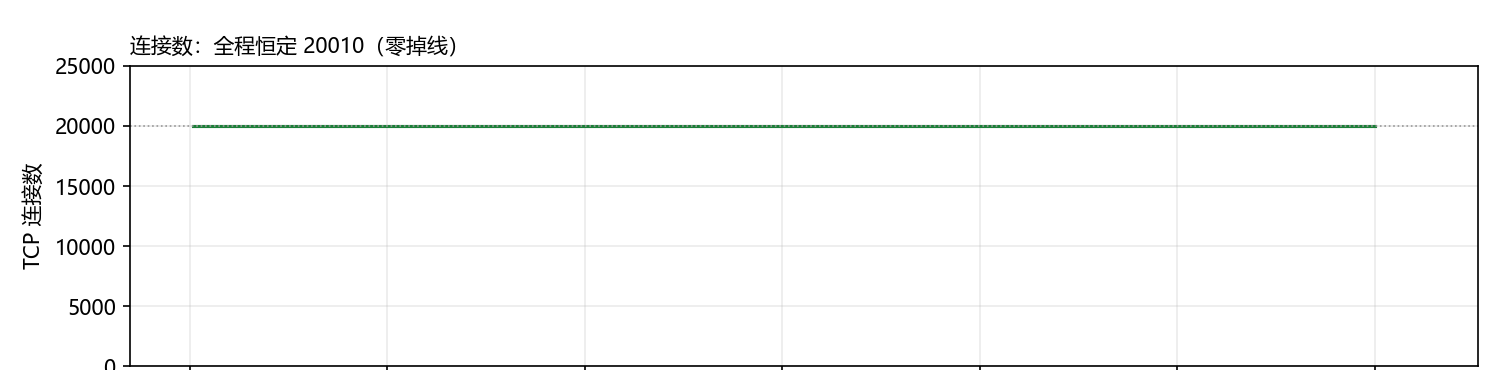
\includegraphics[width=0.88\textwidth, height=0.32\textheight, keepaspectratio]{images/exp_stress_conn.png}\\[8pt]
    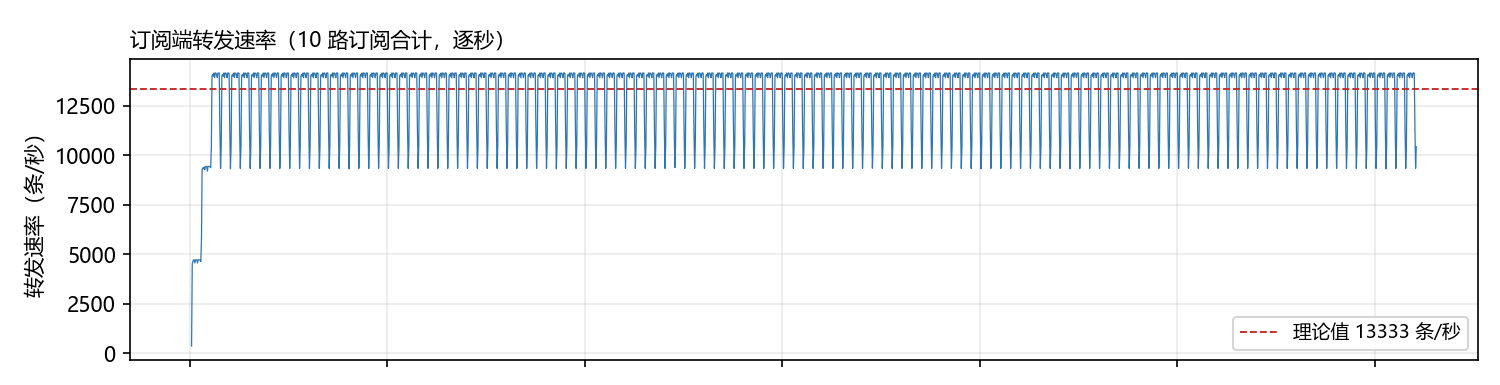
\includegraphics[width=0.88\textwidth, height=0.32\textheight, keepaspectratio]{images/exp_stress_tput.png}
  \end{center}
\end{frame}

\begin{frame}{实测佐证 · 实景压测（2/2）：资源占用极低}
  \vspace{4pt}
  \begin{center}
    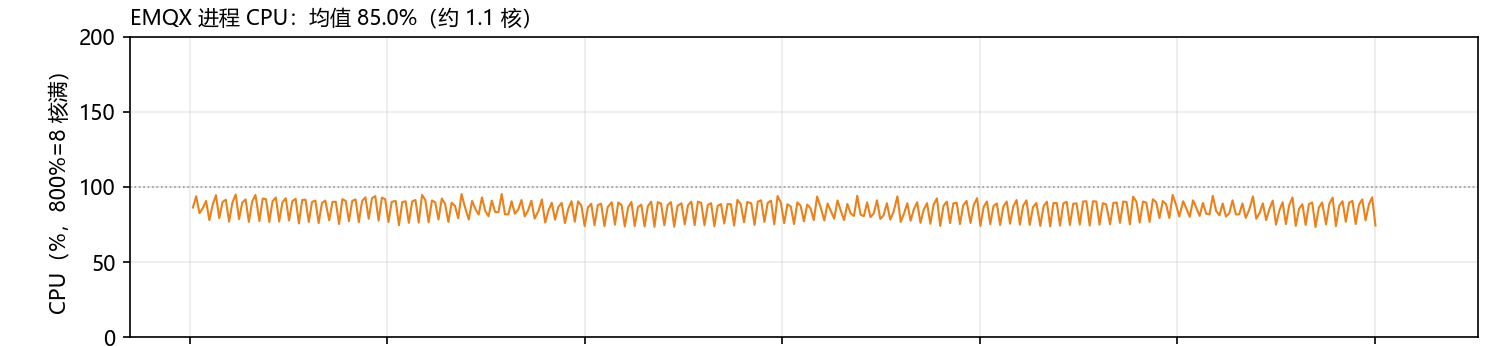
\includegraphics[width=0.88\textwidth, height=0.32\textheight, keepaspectratio]{images/exp_stress_cpu.png}\\[8pt]
    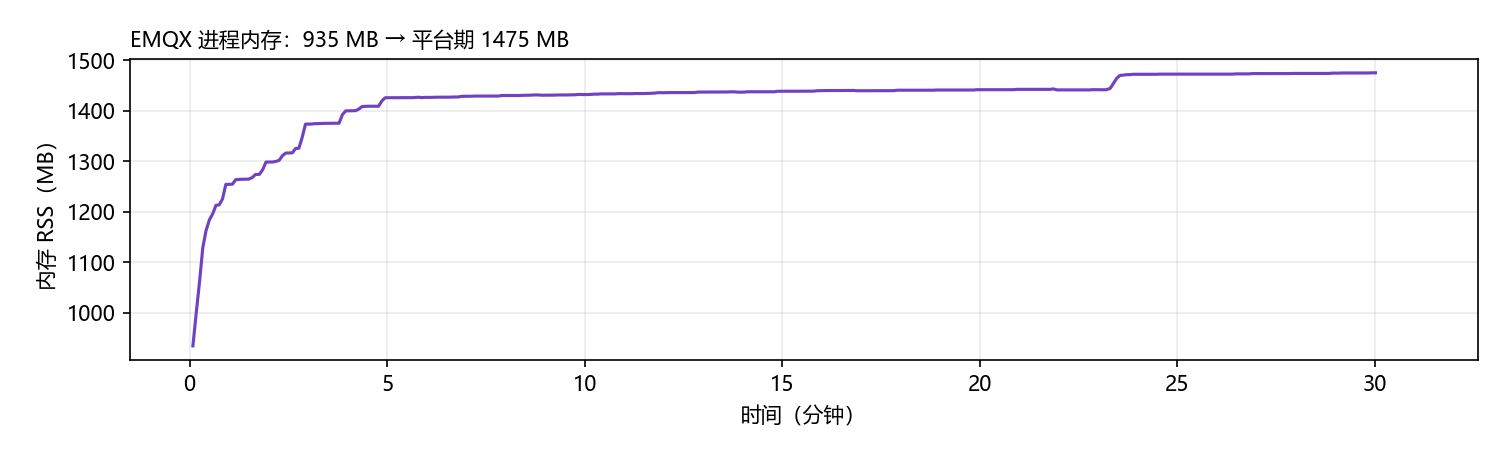
\includegraphics[width=0.88\textwidth, height=0.32\textheight, keepaspectratio]{images/exp_stress_mem.png}
  \end{center}
  \takeaway{2 万连接满载仅 CPU 约 1.1 核 · 内存约 1.5 GB —— 资源占用极低，与容量建模预测吻合}
\end{frame}

% ============================================================
\begin{frame}[standout]
  四、现场演示
\end{frame}

\begin{frame}{现场演示：2 万节点中的“一个”}
  \vspace{10pt}
  \begin{center}
    \begin{tikzpicture}[
        box/.style={draw=black!50, rounded corners=2pt, fill=black!4, align=center,
                    minimum height=0.85cm, inner sep=5pt, font=\scriptsize},
        hub/.style={box, fill=mLightBrown!12, draw=mLightBrown},
        arr/.style={-{Stealth[length=2mm]}, black!55, semithick}]
      \node[box] (esp) {ESP32 节点};
      \node[box, right=1.1cm of esp] (ap) {Wi-Fi AP};
      \node[hub, right=1.1cm of ap] (br) {EMQX};
      \node[box, right=1.1cm of br] (web) {监控端实时刷新};
      \draw[arr] (esp) -- (ap); \draw[arr] (ap) -- (br); \draw[arr] (br) -- (web);
    \end{tikzpicture}
  \end{center}
  \vspace{8pt}
  {\footnotesize
  \begin{enumerate}\itemsep=4pt
    \item 启动 EMQX → ESP32 上传 → 监控端实时显示各节点数据与在线状态
    \item 打开计算器，输入 2 万节点，当场算出 2核4G 配置与成本
  \end{enumerate}}
  \vspace{4pt}
  \hfill{\footnotesize\color{black!55} 现场录屏兜底 · 模拟节点可顶替}
\end{frame}

% ============================================================
\begin{frame}{总结与展望}
  \vspace{6pt}
  \begin{columns}[T]
    \begin{column}{0.48\textwidth}
      \textbf{完成度（对照指标）}
      {\footnotesize
      \begin{itemize}\itemsep=4pt
        \item[$\checkmark$] 到达率 / 延迟 / 重连 全部达标
        \item[$\checkmark$] 需求驱动的成本建模 + 计算器
        \item[$\checkmark$] ESP32 真机长时验证打通链路
      \end{itemize}}
    \end{column}
    \begin{column}{0.48\textwidth}
      \textbf{展望}
      {\footnotesize
      \begin{itemize}\itemsep=4pt
        \item 数据持久化与告警
        \item 多监控端共享订阅降带宽
        \item 边缘聚合下沉、更大规模
      \end{itemize}}
    \end{column}
  \end{columns}
  \takeaway{不堆最强，而是针对校园场景求出满足需求与 QoS 的最低成本方案——方案 + 实验 + 计算器 + 真机闭环}
\end{frame}

\begin{frame}[standout]
  谢谢各位老师\\[6pt]
  {\small 恳请批评指正}
\end{frame}

\end{document}
